\sec{Báze}
V $d$-rozměrném prostoru jsou křivočaré souřadnice v bodě $\vector{x}=(x^{1},x^{2},\dotsc,x^{d})$ zadány funkcemi
\begin{equation}
    \label{eq:qx}
    q^{i}=q^{i}(\vector{x}),
\end{equation}
kde $i=1,\dotsc,d$ a $x^{1},x^{2},\dotsc,x^{d}$ jsou (lokálně definované) kartézské souřadnice.
Bázi \emph{(kovariantní)}\index{báze!kovariantní} v kartézském systému označíme $\vector{e}_{(i)}$, 
takže lze psát\footnote{
    \emph{Einsteinova sčítací konvence:}\index{Einsteinova sčítací konvence}
    Pokud se ve vzorci vyskytnou dva stejně označené indexy, z nichž jeden je nahoře a druhý dole, přes indexy se sčítá:
    \begin{equation}
        x^{i}\vector{e}_{(i)}\equiv\sum_{i=1}^{d}x^{i}\vector{e}_{(i)}.
    \end{equation}
}
\begin{equation}
    \vector{x}=x^{i}\vector{e}_{(i)}\,,
\end{equation}
kde $x^{i}$ jsou \emph{kontravariantní} složky vektoru $\vector{x}$.

\begin{figure}[!h]
    \centering
    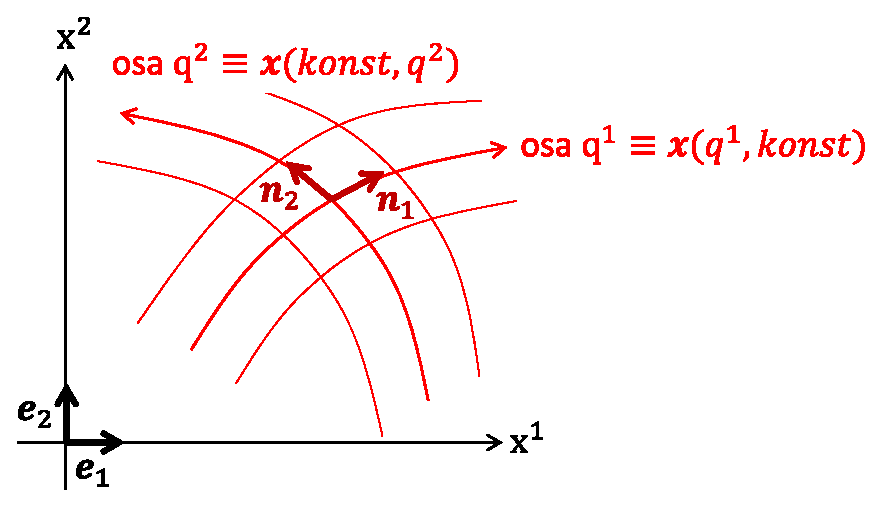
\epsfig{file=figures/coordinates.eps,width=0.66\linewidth}
    \caption{
        Ilustrace souřadnicového systému a lokální báze v křivočarých souřadnicích 
        $(q^{1},q^{2})$.
    }
    \label{fig:CurvilinearCordinates}
\end{figure}

Za předpokladu, že transformace~\eqref{eq:qx} je invertibilní, tj. že existuje inverzní transformace
\begin{equation}
    \label{eq:xq}
    x^{i}=x^{i}(\vector{q}),
\end{equation}
lze v bodě $\vector{x}$ zavést novou bázi ve směru tečen k jednotlivým souřadnicovým čarám $\axis{q}^{i}$, viz obrázek~\ref{fig:CurvilinearCordinates}\footnote{
    Souřadnicová čára $\axis{q}^{i}$ procházející bodem $\vector{Q}=(Q^{1},Q^{2},\dotsc,Q^{d})$ je definována jako čára $\axis{q}^{i}\equiv\vector{x}(q^{1}=Q^{1},\dotsc,q^{i},\dotsc,q^{d}=Q^{d})$ (tento zápis vyjadřuje, že se mění pouze souřadnice $q^{i}$, ostatní souřadnice zůstávají konstantní).
}:
\begin{equation}
    \label{eq:Vectorn}
    \vector{n}_{(i)}=\partialderivative{\vector{x}}{q^{i}}=\partialderivative{x^{j}}{q^{i}}\vector{e}_{(j)}\,;
\end{equation}
jednotlivé složky bázových vektorů $\vector{n}_{(i)}$ tedy jsou
\begin{equation}
    n_{(i)}^{j}=\partialderivative{x^{j}}{q^{i}}\,.
\end{equation}
Je třeba mít na paměti, že zatímco bázové vektory $\vector{e}_{(i)}$ jsou konstantní, bázové vektory $\vector{n}_{(i)}$ obecně závisejí na místě v prostoru: 
$\vector{n}_{(i)}=\vector{n}_{(i)}(\vector{q})$.
